%!TEX encoding = UTF-8 Unicode
% $Id: 24-prolog.tex 18 2014-03-12 22:35:24Z binghe $

\chapter{Prolog}
\label{chap:prolog}
\index{Prolog}

本章将介绍如何编写嵌入式的~Prolog 解释器。
第~\ref{chap:a_query_compiler} 章中已经展示了编写数据库查询语
句编译器的方法,这里我们再加入一个新的元素\index{Prolog!conceptual ingredients}:规则。有了规则,就可以根据已有的知识
通过推理得到新知。
一组规则定义了表明事实之间相互蕴含关系的一棵树。由于这棵树可能包含无限多的事实,所以我们必须使用非确定性的搜索。

Prolog 是嵌入式语言的一个极好的例子。它融合了三个元素:模式匹配,非确定性,
规则。其中,前两个元素在第~\ref{chap:destructuring} 章和
第~\ref{chap:nondeterminism} 章曾分别介绍过。把~Prolog 建立在
模式匹配和非确定性选择操作的基础之上,我们可以得到一个真正的,多层的,自底向
上的系统\index{bottom-up design 自底向上的设计!multilayer 多层的}。图~(\ref{fig:layers_of_abstraction}) 展示了有关几个抽象层的结构。

\begin{figure}
  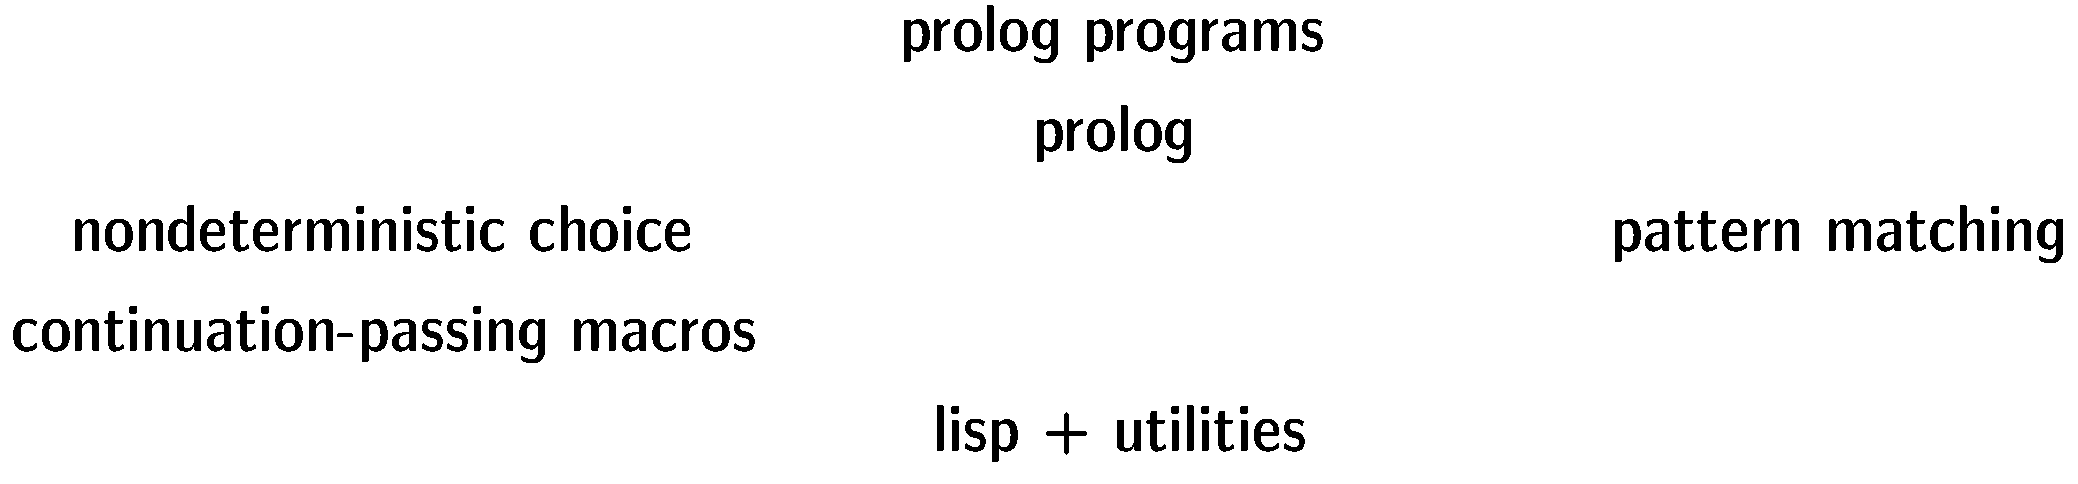
\includegraphics[width=.98\textwidth]{layers.pdf}
  \caption{抽象层}
  \label{fig:layers_of_abstraction}
\end{figure}

本章的第二个目标是学习~Prolog。对于经验丰富的程序员来说,简要地说明一
下其实现方式可能会更有助于讲解这门语言。而用~Lisp 实现~Prolog 非常有趣,因为
在这过程中能够发掘出这两者间的共同点。


\section{概念}
\label{sec:prolog:concepts}

第~\ref{chap:a_query_compiler} 章介绍了如何写一个能接受复杂查询语句的
数据库系统,这个系统能自动生成所有满足查询条件的绑定。在下例中,(调
用~\verb|clear-db| 之后),我们声明两个事实,然后对数据库进行查询:
\begin{lstlisting}
> (fact painter reynolds) 
(REYNOLDS) 
> (fact painter gainsborough) 
(GAINSBOROUGH) 
> (with-answer (painter ?x) 
    (print ?x)) 
GAINSBOROUGH 
REYNOLDS 
NIL 
\end{lstlisting}

从概念上说,Prolog~是一个~``附有规则的数据库程序''。它不仅仅能够直接从
数据库中查找匹配的数据来满足查询语句,还能够从已知的事实~(数据) 中推导
出匹配的数据。例如,若有如下的规则:

\prule
{\texttt{(hungry ?x)} and \texttt{(smells-of ?x turpentine)}}
{\texttt{(painter ?x)}}
则,只要数据库中存在~\texttt{(hungry raoul)} 和~\texttt{(smells-of raoul
  turpentine)} 这两个事实,那么~\texttt{?x = raoul} 就能满足查询语
句~\texttt{(painter ?x)},即使数据库中没有~\texttt{(painter raoul)}
这个事实。

在~Prolog 中,规则的~``if'' 部分被称作~\emph{body}\index{body (of a rule)},``then'' 部分被称
作~\emph{head}。(在逻辑中,它们分别叫做\emph{前提}~(\emph{antecedent})\index{antecedent 前提,前
件,先决条件} 和\emph{推论}~(\emph{consequent})\index{consequent 推论,结果},不过用不同的名字也好,
能强调~Prolog 的推导不同于逻辑的推导)。在我们试图生成查询的绑定
时\footnote{这章的许多概念,比如~binding 的含义,在
  第~\ref{sec:destructuring:matching} 节已经说明。},
程序首先检查规则的~head,如果~head 能满足查询,那么程序会做出
响应,为~body 建立各种绑定。根据定义,如果绑定满足~body,
那么它也满足~head。\index{rules!structure of}

在规则的~\emph{body} 中用到的各种事实可能会转而由其他规则中推演得出。例如:

\prule
{\texttt{(gaunt ?x)} or \texttt{(eats-ravenously ?x)}}
{\texttt{(hungry ?x)}}
规则也可以是递归的,例如:

\prule
{\texttt{(surname ?f ?n)} and \texttt{(father ?f ?c)}}
{\texttt{(surname ?c ?n)}}

如果~Prolog 能在种种规则中找到一条通往已知事实的路径,它便会为该查询建立各
种绑定。因而,它实质上是一个搜索引擎:它遍历由各种规则形成的逻辑蕴含树,
寻找一条通往事实的成功之路。

虽然规则和事实听上去像两回事,其实它们在概念上是可以互
换的\pozhehao{}规则可以被看作虚拟事实\index{rules!as virtual facts}。如果我们希望我们的数据库能够反映出
“凶猛的大型动物是稀有的”这个发现,我们可以寻找所有
的~\emph{x},令~\emph{x} 满足~\texttt{(species $x$)},\texttt{(big
  $x$)} 和~\texttt{(fierce $x$)} 这些事实,找到的话就加上一个新的事实~\texttt{(rare
  $x$)}。如果定义下面的规则:
\prule
{\texttt{(species ?x)} and \texttt{(big ?x)} and \texttt{(fierce ?x)}}
{\texttt{(rare ?x)}}
就会得到相同的效果,而无需在数据库中加入所有的~\texttt{(rare x)} 事实。
我们甚至可以定义能推出无穷个事实的规则。因此,在回应查询的时候,我们通过使用规则,
用额外的数据处理作为代价,缩小了数据库的规模。

另一方面,事实则是规则的一种退化形式。任一事实~\emph{F} 的效用,都可以用一个~\emph{body} 恒为真的规则来达到,
如下:
\prule
{true}
{\emph{F}}
为了简化实现,我们将利用这个性质,并用~bodyless rules\index{Prolog!rules!bodyless} 来表达事实。\note{323}

\section{解释器}
\label{sec:prolog:an_interpreter}
第~\ref{sec:destructuring:matching} 节展示了两种定义~\texttt{if-match}
的方式,前一种简洁但效率低下,后来者由于在编译期完成了大量工作,因而速度有很大的提高。这里,我们将沿用这个策略。
为了便于引出相关的几个话题,我们先从一个简单的解释器开始,然后再介绍如何把同一程序写得更加高效。

\begin{figure}
\begin{lstlisting}
(defmacro with-inference (query &body body)
 `(progn
    (setq *paths* nil)
    (=bind (binds) (prove-query ',(rep_ query) nil)
      (let ,(mapcar #'(lambda (v)
                         `(,v (fullbind ',v binds)))
                     (vars-in query #'atom))
        ,@body
        (fail)))))

(defun rep_ (x)
  (if (atom x)
      (if (eq x '_) (gensym "?") x)
      (cons (rep_ (car x)) (rep_ (cdr x)))))

(defun fullbind (x b)
  (cond ((varsym? x) (aif2 (binding x b)
                            (fullbind it b)
                            (gensym)))
        ((atom x) x)
        (t (cons (fullbind (car x) b)
                 (fullbind (cdr x) b)))))

(defun varsym? (x)
  (and (symbolp x) (eq (char (symbol-name x) 0) #\?)))

\end{lstlisting}
  \caption{Toplevel 宏}
  \label{fig:prolog:toplevel_macro}
  \index{rep\_@\texttt{rep\_}}
  \index{with-inference@\texttt{with-inference}}
  \index{fullbind@\texttt{fullbind}}
\end{figure}

图~\ref{fig:prolog:toplevel_macro}--\ref{fig:code_involving_rules} 包含了一个
简单的~Prolog 解释器。它能接受与第~\ref{sec:a_query_interpreter} 节查询
解释器相同的输入,但使用的是规则而非数据库来生成绑定。查询解释器是通过
宏~\texttt{with-answer} 来调用的,我们的~Prolog 解释器的接口也打算采用
一个类似的宏,称其为~\texttt{with-inference}。犹如~\texttt{with-answer},
\texttt{with-inference} 的输入是一个查询语句
和一组~Lisp 表达式。查询语句中的变量是以问号开头的符号,例如:
\begin{lstlisting}
(with-inference (painter ?x)
  (print ?x))
\end{lstlisting}
\texttt{with-inference} 的一个调用会展开成一段代码,该代码则将~Lisp 表
达式应用于生成的绑定并求值。比如上面那段代码,会把所有能导
出~\texttt{(painter $x$)} 的~\emph{x} 打印出来。\note{325}

图~\ref{fig:prolog:toplevel_macro} 给出了~\texttt{with-inference} 的定
义,及其生成绑定所需的函数。\texttt{with-answer} 和~\texttt{with-inference} 有个显著的区别:
前者只是简单地收集所有的有效绑定,而后者则进行非确定性的搜索。\index{iteration!vs. nondeterministic choice}我们可
以在~\texttt{with-inference} 的定义里注意到这一点:它没有展开成循环\index{iteration!without loops},而
是展开成了一段能返回一组绑定的代码,紧接着是一个~\texttt{fail} 用来重启下
个搜索。这无形中给我们带来了迭代结构。比如:
\begin{lstlisting}
> (choose-bind x '(0 1 2 3 4 5 6 7 8 9)
    (princ x)
    (if (= x 6) x (fail)))
0123456
6
\end{lstlisting}

函数~\texttt{fullbind} 则点出了~\texttt{with-answer} 和~\texttt{with-inference} 的又一不同之处,
沿着规则往回跟踪,我们可以建立一系列绑定\pozhehao{}变量的绑定是其他变量组成的列
表。要使用该查询语句的结果,我们需要一个递归函数来帮我们找到相应的绑定。
这就是~\texttt{fullbind} 的目的,例如:
\begin{lstlisting}
> (setq b '((?x . (?y . ?z)) (?y . foo) (?z . nil)))
((?X ?Y . ?Z) (?Y . FOO) (?Z))
> (values (binding '?x b))
(?Y . ?Z)
> (fullbind '?x b)
(FOO)
\end{lstlisting}

查询语句的绑定的是由~\texttt{with-inference} 展开式中的~\texttt{prove-query}
生成的。图~\ref{fig:interpretation_of_queries} 给出了这个函数的定义及其组成部分。
这段代码和第~\ref{sec:a_query_interpreter} 节中描述的
查询解释器结构相同。两者都用相同的函数用于匹配,只不过查询解释器
用~mapping 和迭代,而~Prolog 解释器则用等价的~\emph{choose}。

\begin{figure}
\begin{lstlisting}
(=defun prove-query (expr binds)
  (case (car expr)
    (and (prove-and (cdr expr) binds))
    (or  (prove-or (cdr expr) binds))
    (not (prove-not (cadr expr) binds))
    (t   (prove-simple expr binds))))

(=defun prove-and (clauses binds)
  (if (null clauses)
      (=values binds)
      (=bind (binds) (prove-query (car clauses) binds)
        (prove-and (cdr clauses) binds))))

(=defun prove-or (clauses binds)
  (choose-bind c clauses
    (prove-query c binds)))

(=defun prove-not (expr binds)
  (let ((save-paths *paths*))
    (setq *paths* nil)
    (choose (=bind (b) (prove-query expr binds)
              (setq *paths* save-paths)
              (fail))
            (progn
              (setq *paths* save-paths)
              (=values binds)))))

(=defun prove-simple (query binds)
  (choose-bind r *rlist*
    (implies r query binds)))

\end{lstlisting}
  \caption{查询语句的解释}
  \label{fig:interpretation_of_queries}
\end{figure}

不过,使用非确定性搜索替代迭代的方式确实让解释否定\index{negation!in Prolog}的查询语句变得更难了。例如下
面的查询语句:
\begin{lstlisting}
(not (painter ?x))
\end{lstlisting}
查询解释器只需要为~\verb|(painter ?x)| 建立绑定,如果找到任意的绑定则
返回~\texttt{nil}。而使用非确定性搜索的话,就必须更加小心,因为我们不希
望~\texttt{(painter ?x)} 在~\verb|not| 的作用域之外~fail,同时~(如
果~\texttt{(painter ?x)} 为真) 我们也不希望保留其剩下还未探索的路径。所
以,\texttt{(painter ?x)} 的判断被应用在一个临时的空的搜索路径的环境中。
当判断结束时,会恢复原先的路径。

它们之间的另一区别在于对简单模板的解释\pozhehao{}类似
于~\texttt{(painter ?x)} 的仅仅由一个谓词和几个参数组成的表达式。当查询
解释器对简单模板生成绑定时,它调
用~\texttt{lookup}~(第~\pageref{fig:query_interpreter} 页)。
在~Prolog 解释器中,我们必须找到所有规则所能推导出的绑定,因
此~\texttt{lookup} 已不适用。

\begin{figure}
\begin{lstlisting}
(defvar *rlist* nil)

(defmacro <- (con &rest ant)
  (let ((ant (if (= (length ant) 1)
                 (car ant)
                 `(and ,@ant))))
    `(length (conc1f *rlist* (rep_ (cons ',ant ',con))))))

(=defun implies (r query binds)
  (let ((r2 (change-vars r)))
    (aif2 (match query (cdr r2) binds)
          (prove-query (car r2) it)
          (fail))))

(defun change-vars (r)
  (sublis (mapcar #'(lambda (v)
                      (cons v (symb '? (gensym))))
                  (vars-in r #'atom))
          r))
\end{lstlisting}
  \caption{包含规则的代码}
  \label{fig:code_involving_rules}
\end{figure}

\begin{figure}
  \begin{tabular}{ll}
    $\langle\mathrm{rule}\rangle$     & \texttt{: (<- $\langle\mathrm{sentence}\rangle$ $\langle\mathrm{query}\rangle$)} \\
    $\langle\mathrm{query}\rangle$    & \texttt{: (not $\langle\mathrm{query}\rangle$)} \\
                                      & \texttt{: (and $\langle\mathrm{query}\rangle$*)} \\
                                      & \texttt{: (or $\langle\mathrm{query}\rangle$*)} \\
                                      & \texttt{: $\langle\mathrm{sentence}\rangle$} \\
    $\langle\mathrm{sentence}\rangle$ & \texttt{: ($\langle\mathrm{symbol}\rangle$ $\langle\mathrm{argument}\rangle$*)} \\
    $\langle\mathrm{argument}\rangle$ & \texttt{: $\langle\mathrm{variable}\rangle$} \\
                                      & \texttt{: $\langle\mathrm{symbol}\rangle$} \\
                                      & \texttt{: $\langle\mathrm{number}\rangle$} \\
    $\langle\mathrm{variable}\rangle$ & \texttt{: ?$\langle\mathrm{symbol}\rangle$}
  \end{tabular}
  \caption{规则的语法}
  \label{fig:syntax_of_rules}
\end{figure}

图~\ref{fig:code_involving_rules} 中给出了定义和使用规则的代码。
规则被放在全局列表~\verb|*rlist*| 中。每个规则由~body
和~head 所组成的点对~(dotted pair) 表达。当一个规则被定义后,任一下划线会被
替换为一个唯一的变量。

\verb|<-| 的定义遵循了三个惯例,一般来说,编写这类程序时通常都会采纳这些习惯做法:

\begin{enumerate}
\item 加入新规则的时候,应当把规则放到列表末尾,而不是最前面,这样应用
  规则时的顺序就和定义规则的顺序一致了。
\item 在表示规则的时候,要把~head 放在前面,因为程序查看规则的顺序就是如此。
\item 如果~body 里有多个表达式的话,它们事实上被放在了看不见的~\verb|and|\index{Prolog!rules!implicit conjunction in body} 里面。
\end{enumerate}

在~\verb|<-| 的展开式最外层调用了~\verb|length|,其目的是为了避免在~toplevel 
调用~\verb|<-| 时,打印出巨大的列表。

规则的语法如图~\ref{fig:syntax_of_rules} 所示。规则的~head 必须是一种事实的模式:
一个列表,列表的每个元素都由一个谓词,跟着任意数量的参数。body 可以是任何查询语句,
只要第~\ref{chap:a_query_compiler} 章的查询解释器能读懂它就行。下面是本章前面曾
用过的一个规则:
\begin{lstlisting}
(<- (painter ?x) (and (hungry ?x)
                      (smells-of ?x turpentine)))
\end{lstlisting}
或直接
\begin{lstlisting}
(<- (painter ?x) (hungry ?x)
                 (smells-of ?x turpentine))
\end{lstlisting}
和查询解释器一样,类似~\verb|turpentine| 的参数不会被求值,
所以它们没有必要被 quoted。

当我们让~\verb|prove-simple| 为某个查询生成绑定时,它的非确定地选择一条规则,并把该规则和查询一同送给
~\verb|implies|。下一个函数则试图把查询和规则的~head 匹配起来。一旦匹配成功,\verb|implies| 将会调用~\verb|prove-query|,
让它帮助为~body 建立绑定。用这种方法,我们递归搜索逻辑蕴含树。

\verb|change-vars| 函数把规则中所有的变量换成新生成的。
如果在某个规则里使用了~\verb|?x|,那么这个~\verb|?x| 是和其它规则里面的~\verb|?x| 是没有关系的。为了避免现有绑定之间发生冲突,
每应用一条规则,都会调用~\verb|change-vars|。

为了给用户提供方便,这里可以把~\verb|_|
(下划线)\index{\_@\texttt{\_}} 用作规则里的通配符变量。在定义规则的时候,
会调用函数~\verb|rep_|,它把每个下划线都替换成真正的变量。下划线也可以用在传给
~\verb|with-inference| 的查询里面。


\section{规则}
\label{sec:prolog:rules}

本节将介绍如何为我们的~Prolog 编制规则。先以第~\ref{sec:prolog:concepts} 节中的两条规则为例:
\begin{lstlisting}
(<- (painter ?x) (hungry ?x)
                 (smells-of ?x turpentine))

(<- (hungry ?x) (or (gaunt ?x) (eats-ravenously ?x)))
\end{lstlisting}
倘若我们同样也断言了~(assert) 下面几个事实:
\begin{lstlisting}
(<- (gaunt raoul))
(<- (smells-of raoul turpentine))
(<- (painter rubens))
\end{lstlisting}
它们将根据其定义的顺序\index{Prolog!rules!order of},来决定要生成的绑定:
\begin{lstlisting}
> (with-inference (painter ?x)
    (print ?x))
RAOUL
RUBENS
@
\end{lstlisting}
\verb|with-inference| 宏和~\verb|with-answer| 一样,对变量绑定有着相同限制~(见第~\ref{sec:the_database} 节)。

我们能写出这样一种规则,它意味着:对所有可能的绑定,都可以令给定形式的事实为真。
这并非不可能。比如说,如果有变量出现在规则的~head 里,但却在~body 里销声匿迹。这种规则就能满足要求。
下面的规则
\begin{lstlisting}
(<- (eats ?x ?f) (glutton ?x))
\end{lstlisting}
说道:如果~\verb|?x| 是个吃货~(glutton),那么~\verb|?x| 就来者不据,照单全收。因为~\verb|?f| 在~body 里没有出现,
所以,只消为~\verb|?x| 设立一个绑定,就能证明任意形如~\texttt{(eats ?x $y$)} 的事实。如果我们用一个字面值作为~\verb|eats| 的第二个参数,
进行查询,
\begin{lstlisting}
> (<- (glutton hubert))
7
> (with-inference (eats ?x spinach)
    (print ?x))
HUBERT
@
\end{lstlisting}
那么任何字面值都能满足要求。如果把一个变量作为第二个参数的话:

\begin{lstlisting}
> (with-inference (eats ?x ?y)
    (print (list ?x ?y)))
(HUBERT #:G229)
@
\end{lstlisting}
我们会得到一个~gensym。在查询中把~gensym 作为变量的绑定返回,这表示任意值都能令事实为真。
在编程序的时候,可以显式地利用这一惯例:
\begin{lstlisting}
> (progn
    (<- (eats monster bad-children))
    (<- (eats warhol candy)))
9
> (with-inference (eats ?x ?y)
    (format t "~A eats ~A.~%"
            ?x
            (if (gensym? ?y) 'everything ?y)))
HUBERT eats EVERYTHING.
MONSTER eats BAD-CHILDREN.
WARHOL eats CANDY.
@
\end{lstlisting}
最后,如果我们想要指定一个特定形式的事实对任意参数都为真,那么可以令其~body 为无参数的合取式。
\verb|(and)| 表达式和永真式的事实,其行为表现是一样的。由于在~\verb|<-| 宏中~(图~\ref{fig:code_involving_rules}),
body 的缺省设置就是~\verb|(and)|,所以对于这种规则,我们可以直接略去其~body:
\begin{lstlisting}
> (<- (identical ?x ?x))
10
> (with-inference (identical a ?x)
    (print ?x))
A
@
\end{lstlisting}

若是读者已经粗通~Prolog,就可以看出图~\ref{fig:prolog_syntax_equivalence} 展示了把~Prolog 语法转换
到我们程序语法的过程。照老习惯,第一个~Prolog 程序往往是~\verb|append|,它可以写成图~\ref{fig:prolog_syntax_equivalence} 结尾的那样。在一次~append 中,两个较短的列表被并成一个更长的列表。Lisp 的函数~\verb|append| 把两个短列表作为参数,而将长列表当成
返回值。Prolog 的~\verb|append| 更通用一些。图~\ref{fig:prolog_syntax_equivalence} 中的两条规则定义了一个程序,
只要传入任意两个相关的列表,这个程序就能找到第三个。

\begin{figure}
我们的语法和传统的~Prolog 语法间有如下几点区别:
\begin{enumerate}
\item 使用以问号开头的符号,而非大写字母来表示变量。因为~Common Lisp 缺省是不区分大小写的\index{case-sensitivity}\index{Common Lisp!case-sensitivity of}\index{Prolog!case-sensitivity of},所以用大写字母的话可能会得不偿失。
\item \verb|[ ]| 变成了~\verb|nil|。
\item 形如~\verb+[x | y]+ 的表达式成了~\verb|(x . y)|。
\item 形如~\verb|[x, y, ...]| 的表达式成了~\verb|(x y...)|。
\item 断言被挪到了括弧里面,而且用来分隔参数的逗号也被去掉了:\texttt{$pred$($x$, $y$, ...)} 成了~\texttt{($pred$ $x$ $y$ ...)}。
\end{enumerate}

于是乎,Prolog 对~\verb|append| 的定义:
\begin{lstlisting}
append([ ], Xs, Xs).
append([X | Xs], Ys, [X | Zs]) <- append(Xs, Ys, Zs).
\end{lstlisting}
就成了下面的模样:
\begin{lstlisting}
(<- (append nil ?xs ?xs))
(<- (append (?x . ?xs) ?ys (?x . ?zs))
    (append ?xs ?ys ?zs))
\end{lstlisting}
  \caption{和~Prolog 语法的对应关系}
  \label{fig:prolog_syntax_equivalence}
  \index{Prolog!syntax of}
  \index{append@\texttt{append}!Prolog implementation}
\end{figure}

\begin{lstlisting}
> (with-inference (append ?x (c d) (a b c d))
    (format t "Left: ~A~%" ?x))
Left: (A B)
@
> (with-inference (append (a b) ?x (a b c d))
    (format t "Right: ~A~%" ?x))
Right: (C D)
@
> (with-inference (append (a b) (c d) ?x)
    (format t "Whole: ~A~%" ?x))
Whole: (ABCD)
@
\end{lstlisting}
不仅如此,如果给出了最后一个列表,它还能找出前两个列表所有可能的组合:
\begin{lstlisting}
> (with-inference (append ?x ?y (a b c))
    (format t "Left: ~A Right: ~A~%" ?x ?y))
Left: NIL Right: (A B C)
Left: (A) Right: (B C)
Left: (A B) Right: (C)
Left: (A B C) Right: NIL
@
\end{lstlisting}
\verb|append| 这个例子揭示出了~Prolog 和其它语言之间的天差地别。一组~Prolog 规则不一定非要
推出某个特定的值。这些规则也可以给出一些\emph{约束}~(constraints),而
这些约束和由程序其他部分生成的约束一同,将能得出一个特定的值。举例来说,如果这样定义~\verb|member|:
\begin{lstlisting}
(<- (member ?x (?x . ?rest)))
(<- (member ?x (_ . ?rest)) (member ?x ?rest))
\end{lstlisting}
就能用它判断列表的成员关系,和~Lisp 的函数~\verb|member| 的用法一模一样:
\begin{lstlisting}
> (with-inference (member a (a b)) (print t))
T
@
\end{lstlisting}
不过,我们也可以用它新建一个成员关系的约束,这个约束和其他约束一起,同样可以得出
一个特定的列表。如果我们手里还有个谓词叫~\verb|cara|
\begin{lstlisting}
(<- (cara (a _)))
\end{lstlisting}
任意一个有两个元素的列表,只要其~car 为~\verb|a|,那么这个事实就为真。这样,有了这个谓词和~\verb|member|,
就有了充足的约束条件,可以让~Prolog 为我们想出一个确定的答案了:
\begin{lstlisting}
> (with-inference (and (cara ?lst) (member b ?lst))
    (print ?lst))
(A B)
@
\end{lstlisting}

例子很简单,但是其中的道理在编写更大规模的程序时也一样适用。
无论何时,只要我们想通过把部分结果组合到一起的方式来编写程序,那么就能用上~Prolog。
事实上借助这种方式可以表达很多类型的问题:比如说,图~\ref{fig:quicksort} 就展示了一个排序算法,
这个排序算法是由一组对计算结果的约束来表示的。

\section{对于非确定性的需求}
\label{sec:the_need_for_nodeterminism}
\index{Prolog!nondeterminism in}

第~\ref{chap:nondeterminism} 章解释了确定性和非确定性搜索的区别所在。
使用确定性搜索的程序能接受一个查询,并生成所有满足这个查询的结果。而用非确定性搜索
的程序则会借助~\emph{choose},每次生成一个结果,如果用户需要更多的结果,
那么它会调用~\emph{fail},来重新启动这个搜索过程。

如果我们手中的规则得出的都是有限大小的绑定集合,而且我们希望一次性的得到所有这些绑定,
那么就没有理由用非确定性搜索。倘若我们的查询会产生无穷多的绑定,而我们要的只是其中的一个
有限子集,那么这两种搜索策略的区别就一目了然了。比如说,下面的规则
\begin{lstlisting}
(<- (all-elements ?x nil))
(<- (all-elements ?x (?x . ?rest))
    (all-elements ?x ?rest))
\end{lstlisting}
蕴含所有形如~\verb|(all-elements x y)| 的事实,$y$ 的每一个成员都等于~$x$。
不用回溯的话,我们有能力处理类似下面的查询:
\begin{lstlisting}
(all-elements a  (a a a))
(all-elements a  (a a b))
(all-elements ?x (a a a))
\end{lstlisting}
然而,有无数多的~\verb|?x| 可以满足~\verb|(all-elements a ?x)| 这个查询,比如:\verb|nil|、
\verb|(a)|、\verb|(a a)|,等等。要是想用迭代的方式为这个查询生成答案,
那么这个迭代就会永不休止,一直运行下去。就算我们弱水三千只取一瓢饮,在这无穷多的答案中仅仅要一个,
如果算法的实现在走到下一个~Lisp 表达式之前,必须为查询准备好所有的绑定,那么我们永远等不到那一天,
更不用说得到答案了。

这就是为什么~\verb|with-inference| 把绑定的产生过程和其~body 的求值过程交错进行的原因。
由于查询可能会对应无穷多的答案,所以唯一的办法只能是每次产生一个答案,并通过重启前被暂停的
搜索来取得新的答案。因为我们的程序使用了~\emph{choose} 和~\emph{fail},所以它能够解决下面的问题:
\begin{lstlisting}
> (block nil
    (with-inference (all-elements a ?x)
      (if (= (length ?x) 3)
          (return ?x)
          (princ ?x))))
NIL(A)(A A)
(A A A)
\end{lstlisting}

和所有的~Prolog 实现一样,我们也是借助带回溯的深度优先搜索来模拟非确定性的。
从理论上而言,``逻辑程序'' 是由真正的非确定性驱动的。而实际上,各家~Prolog 实现却常常用的是深度优先搜索。
这个选择非但没有造成不便,相反,深度优先版的非确定性是标准的~Prolog 程序赖以正常工作的基础。
在使用真实非确定性的世界里,下面的查询
\begin{lstlisting}
(and (all-elements a ?x) (length ?x 3))
\end{lstlisting}
是有答案的,但是在得到这个答案之前,你必须先等到海枯石烂。

Prolog 使用深度优先搜索实现非确定性,不仅如此,它使用的深度优先还和第
~\pageref{fig:scheme_implementation_of_choose_and_fail} 页中
定义的版本等价。正如我们在那里提到的,这个实现是不能保证终止的。所以
~Prolog 程序员必须采取专门的措施,避免在搜索空间里面产生环。举例来说,
如果我们以相反的顺序定义~\verb|member|\index{Prolog!rules!left-recursive}
\begin{lstlisting}
(<- (member ?x (_ . ?rest)) (member ?x ?rest))
(<- (member ?x (?x . ?rest)))
\end{lstlisting}
那么照道理来说,其意义应该保持不变,但是作为~Prolog 程序的话,
效果就完全不同了。如果使用~\verb|member| 原来的定义,
那么查询~\verb|(member 'a ?x)|,会得到一系列连绵不绝,无穷多的答案。
但是如果把定义的顺序反过来,则会产生一个无穷递归,一个答案都得不到。

\section{新的实现}
\label{sec:new_implementation}

在这一节,我们会故友重逢,碰到一个熟悉模式的另一实例。在第~\ref{sec:destructuring:matching} 节,
在编完~\verb|if-match| 的最初版本之后,我们发现其实可以把它实现得更快。通过利用编译期的已知信息,
我们本可以写一个新的版本,让它在运行期做更少的事情。后来,在第~\ref{chap:a_query_compiler} 章,
我们经历了同样的问题,不过这一次程序的规模更大。我们把查询解释器换成了一个与之等价,但更高效的版本。
历史将会在我们的~Prolog 解释器上重演。

图~\ref{fig:new_toplevel_macro}, \ref{fig:compilation_of_queries}, \ref{fig:code_for_defining_rules} 一起以另一种方式定义了~Prolog。
宏~\verb|with-inference| 以前只是~Prolog 解释器的接口。它现在成了程序的主要的组成部分。
新程序的结构和原来基本一致,不过在图~\ref{fig:compilation_of_queries} 中定义的函数里面,
只有~\verb|prove| 是在运行期调用的。其他函数则由~\verb|with-inference| 调用,被用来
生成其展开式。

图~\ref{fig:new_toplevel_macro} 中是~\verb|with-inference| 的新定义。和~\verb|if-match| 以及
~\verb|with-answer| 中一样,模式匹配变量在开始的时候会被绑定到~gensym 上,表示它们还没有被匹配过程赋予真正的值。
因而,被~\verb|match| 和~\verb|fullbind| 用来辨别变量的函数~\verb|varsym?|,就需要修改一下,转而检查是否是~gensym。

\verb|with-inference| 调用~\verb|gen-query| (图~\ref{fig:compilation_of_queries}) 的目的是为了生成一部分代码,
这些代码将为查询建立绑定。\verb|gen-query| 要做的的一件事是检查它的第一个参数是不是那种以~\verb|and| 或者~\verb|or| 开头的复杂查询。
这个过程会递归地进行,直至遇到简单查询,这些简单查询会被展开成对~\verb|prove| 的调用。
在原来的实现中,这种逻辑结构是在运行期完成解析的。以前,每次使用规则时,都必须重新分析~body 中的复杂查询。
显然,这毫无必要。因为规则和查询的逻辑结构是事先已知的。针对这个问题,新版的实现把复杂表达式的解析工作移到了编译期。

和原来的实现一样,\verb|with-inference| 表达式展开出的代码会先进行一次查询,
查询中的模式变量所绑定到的值是由规则一一设定的,然后再迭代执行~Lisp 代码。
\verb|with-inference| 的展开式以一个~\verb|fail| 作结,后者会重启之前保存的状态。

图~\ref{fig:compilation_of_queries} 中其他函数会为复杂查询生成对应的展开式\pozhehao{}
即由诸如~\verb|and|、\verb|or| 和~\verb|not| 的操作符结合起来的查询。
倘若有如下的查询
\begin{lstlisting}
(and (big ?x) (red ?x))
\end{lstlisting}
并且,我们希望只有那些能同时~prove 两个合取式的~\verb|?x|,才被带入~Lisp 代码求值。
因此,为了生成~\verb|and| 的展开式,我们把第二个合取式的展开式嵌入到第一个合取式的展开式中。
要是~\verb|(big ?x)| 成功了,就继续尝试~\verb|(red ?x)|,如果后者也成功的话,则对这个~Lisp 表达式进行求值。
如此,整个表达式展开后如图~\ref{fig:expansion_of_a_conjunction} 所示。

\begin{figure}
\begin{lstlisting}
(defmacro with-inference (query &rest body)
  (let ((vars (vars-in query #'simple?)) (gb (gensym)))
    `(with-gensyms ,vars
       (setq *paths* nil)
       (=bind (,gb) ,(gen-query (rep_ query))
         (let ,(mapcar #'(lambda (v)
                           '(,v (fullbind ,v ,gb)))
                       vars)
           ,@body)
         (fail)))))

(defun varsym? (x)
  (and (symbolp x) (not (symbol-package x))))
\end{lstlisting}
\caption{新的~toplevel 宏}
\label{fig:new_toplevel_macro}
\index{varsym?@\texttt{varsym?}!redefined}
\index{with-inference@\texttt{with-inference}!redefined}
\end{figure}

\begin{figure}
\begin{lstlisting}
(defun gen-query (expr &optional binds)
  (case (car expr)
    (and (gen-and (cdr expr) binds))
    (or  (gen-or (cdr expr) binds))
    (not (gen-not (cadr expr) binds))
    (t   `(prove (list ',(car expr)
                      ,@(mapcar #'form (cdr expr)))
               ,binds))))

(defun gen-and (clauses binds)
  (if (null clauses)
      `(=values ,binds)
       (let ((gb (gensym)))
         '(=bind (,gb) ,(gen-query (car clauses) binds)
            ,(gen-and (cdr clauses) gb)))))

(defun gen-or (clauses binds)
  `(choose
    ,@(mapcar #'(lambda (c) (gen-query c binds))
              clauses)))

(defun gen-not (expr binds)
  (let ((gpaths (gensym)))
    `(let ((,gpaths *paths*))
       (setq *paths* nil)
       (choose (=bind (b) ,(gen-query expr binds)
                 (setq *paths* ,gpaths)
                 (fail))
               (progn
                 (setq *paths* ,gpaths)
                 (=values ,binds))))))

(=defun prove (query binds)
        (choose-bind r *rules* (=funcall r query binds)))

(defun form (pat)
  (if (simple? pat)
      pat
      `(cons ,(form (car pat)) ,(form (cdr pat)))))
\end{lstlisting}
\caption{对查询进行的编译处理}
\label{fig:compilation_of_queries}
\end{figure}

\begin{figure}
\begin{lstlisting}
(with-inference (and (big ?x) (red ?x))
  (print ?x))
\end{lstlisting}
  expands into:
\begin{lstlisting}
(with-gensyms (?x)
  (setq *paths* nil)
  (=bind (#:g1) (=bind (#:g2) (prove (list 'big ?x) nil)
                  (=bind (#:g3) (prove (list 'red ?x) #:g2)
                    (=values #:g3)))
     (let ((?x (fullbind ?x #:g1)))
       (print ?x))
     (fail)))
\end{lstlisting}
\caption{合取式的展开}
\label{fig:expansion_of_a_conjunction}
\end{figure}

\verb|and| 意味着嵌入;而~\verb|or| 则意味着~\emph{choose}。有下列查询
\begin{lstlisting}
(or (big ?x) (red ?x))
\end{lstlisting}
两个子查询,如果其中任意一个能建立~\verb|?x| 的绑定,我们将希望 Lisp 表达式使用这些~\verb|?x| 来进行求值。
函数~\verb|gen-or| 会展开成~\verb|choose|,后者会在诸参数的~\verb|gen-query| 中选择一个。
至于~\verb|not|,\verb|gen-not| 基本上和~\verb|prove-not| 同出一辙 (见图~\ref{fig:interpretation_of_queries})。

图~\ref{fig:code_for_defining_rules} 中是定义规则的代码。规则被直接转换成~Lisp 代码,而后者是由
~\verb|rule-fn| 生成的。因为现在~\verb|<-| 把规则展开成了~Lisp 代码,所以如果把一个写满了规则定义
的文件编译了的话,就会让这些规则变成编译过的函数。

当一个~rule-function 收到一个模式时,它会试图把自己所表示规则的~head 与之匹配。如果匹配成功,
这个~rule-function 就会试图为其~body 设立绑定。这个过程和~\verb|with-inference| 的功能基本一致,
而且,事实上~\verb|rule-fn| 会在结束的时候调用~\verb|gen-query|。rule-function 最终会返回一些绑定,
它们是为规则的~head 中出现的变量而设立的。

\begin{figure}
\begin{lstlisting}
(defvar *rules* nil)

(defmacro <- (con &rest ant)
  (let ((ant (if (= (length ant) 1)
                 (car ant)
                 `(and ,@ant))))
    `(length (conc1f *rules*
                     ,(rule-fn (rep_ ant) (rep_ con))))))

(defun rule-fn (ant con)
  (with-gensyms (val win fact binds)
    `(=lambda (,fact ,binds)
       (with-gensyms ,(vars-in (list ant con) #'simple?)
         (multiple-value-bind
             (,val ,win)
             (match ,fact
                    (list ',(car con)
                          ,@(mapcar #'form (cdr con)))
                    ,binds)
           (if ,win
               ,(gen-query ant val)
             (fail)))))))
\end{lstlisting}
\caption{定义规则的代码}
\label{fig:code_for_defining_rules}
\end{figure}

\section{增添~Prolog 特性}
\label{sec:adding_prolog_features}

现有的代码已足以运行绝大多数的``纯''Prolog 程序。最后一步是再加入一些特性,诸如:减枝~(cut)\index{cut}, 数学计算,还有~\textsc{I/O}。

在~Prolog 规则中加入~\emph{cut},就能对搜索树进行剪枝了。通常,
当我们的程序碰到~\verb|fail| 的时候,它会回溯到最后一个选择点。在第~\ref{sec:common_lisp_implementation} 节实现的
~\emph{choose} 中,把历史上的选择点都放到了全局变量~\verb|*paths*| 里。调用~\verb|fail|,会在最新近的一个选择点重新
启动搜索过程,而这个选择点就是~\verb|*paths*| 的~car。cut 让问题更复杂了。当程序遇到~\verb|cut| 时,它会放弃保存在
~\verb|*paths*| 里的一部分最新选择点,具体说,就是在最后一次调用~\verb|prove| 之后保存的选择点。

其结果就是让规则之间互斥。我们可以用~cut 来在~Prolog 程序中达到~case 语句的效果。
举例来说,如果像下面这样定义~\verb|minimum|:
\begin{lstlisting}
(<- (minimum ?x ?y ?x) (lisp (<= ?x ?y)))
(<- (minimum ?x ?y ?y) (lisp (> ?x ?y)))
\end{lstlisting}
它会工作正常,但是比较没有效率。若有下列查询
\begin{lstlisting}
(minimum 1 2 ?x)
\end{lstlisting}

根据第一条规则,Prolog 将会立即建立~\verb|?x = 1|。倘若是人的话,就会到此为止,
但是程序会虚掷光阴,继续从第二条规则那里找寻答案,因为没人告诉它这两条规则是
互斥的。平均情况下,这个版本的~\verb|minimum| 会多做~50\% 的无用功。
如果在第一个测试后面加个~\verb|cut| 就能解决这一问题:
\begin{lstlisting}
(<- (minimum ?x ?y ?x) (lisp (<= ?x ?y)) (cut))
(<- (minimum ?x ?y ?y))
\end{lstlisting}
现在,一旦~Prolog 完成了第一条规则,它就会一路掠过剩下的规则,完成查询,而不是
继续处理下一条规则。
要让我们的程序支持减枝,简直易如反掌。每次在调用
~\verb|prove| 时,当前~\verb|*paths*| 的状态都会被当作参数传进去。如果程序碰到了
~cut,它就把~\verb|*paths*| 设置回上一次当作参数传入的值。
图~\ref{fig:adding_support_for_new_operators-1} 和~\ref{fig:adding_support_for_new_operators-2} 显示了
为了支持减枝,必须改动的部分代码。
(修改过的代码行后面有分号以示区别。并非所有的改动都是由于减枝而造成的。)

仅仅提高程序效率的~cut 叫做~\emph{green cuts}\index{cut!green}。\verb|minimum| 
中的~cut 就是个~green cut。那种会改变程序行为的~cut 则被称为~\emph{red cuts}\index{cut!red}。
比如说,如果我们像下面那样定义谓词~\verb|artist|:
\begin{lstlisting}
(<- (artist ?x) (sculptor ?x) (cut))
(<- (artist ?x) (painter ?x))
\end{lstlisting}
结果就是:如果有雕塑家,那么查询到此结束。如果一个雕塑家都找不到,那么就把画家认作艺术家:
\begin{lstlisting}
> (progn (<- (painter 'klee))
         (<- (painter 'soutine)))
4
> (with-inference (artist ?x)
    (print ?x))
KLEE
SOUTINE
@
\end{lstlisting}
但如果存在雕塑家的话,减枝机制使得推理在处理第一条规则时就会停止:
\begin{lstlisting}
> (<- (sculptor 'hepworth))
5
> (with-inference (artist ?x)
    (print ?x))
HEPWORTH
@
\end{lstlisting}

\begin{figure}
\begin{lstlisting}[escapechar=\~]
(defun rule-fn (ant con)
  (with-gensyms (val win fact binds paths)                 ~\hfill~;
    `(=lambda (,fact ,binds ,paths)                        ~\hfill~;
       (with-gensyms ,(vars-in (list ant con) #'simple?)
         (multiple-value-bind
             (,val ,win)
             (match ,fact
                    (list ',(car con)
                          ,@(mapcar #'form (cdr con)))
                    ,binds)
           (if ,win
               ,(gen-query ant val paths)                  ~\hfill~;
               (fail)))))))

(defmacro with-inference (query &rest body)
  (let ((vars (vars-in query #'simple?)) (gb (gensym)))
    `(with-gensyms ,vars
       (setq *paths* nil)
       (=bind (,gb) ,(gen-query (rep_ query) nil '*paths*) ~\hfill~;
         (let ,(mapcar #'(lambda (v)
                           '(,v (fullbind ,v ,gb)))
                       vars)
           ,@body)
         (fail)))))

(defun gen-query (expr binds paths)                        ~\hfill~;
  (case (car expr)
    (and  (gen-and (cdr expr) binds paths))                ~\hfill~;
    (or   (gen-or (cdr expr) binds paths))                 ~\hfill~;
    (not  (gen-not (cadr expr) binds paths))               ~\hfill~;
    (lisp (gen-lisp (cadr expr) binds))                    ~\hfill~;
    (is   (gen-is (cadr expr) (third expr) binds))         ~\hfill~;
    (cut `(progn (setq *paths* ,paths)                     ~\hfill~;
                 (=values ,binds)))                        ~\hfill~;
    (t   `(prove (list ',(car expr)
                           ,@(mapcar #'form (cdr expr)))
                  ,binds *paths*))))                       ~\hfill~;

(=defun prove (query binds paths)                          ~\hfill~;
   (choose-bind r *rules*
     (=funcall r query binds paths)))                      ~\hfill~;
\end{lstlisting}
  \caption{加入对新操作符的支持}
  \label{fig:adding_support_for_new_operators-1}
  \index{with-inference@\texttt{with-inference}!redefined}
\end{figure}


\begin{figure}
\begin{lstlisting}[escapechar=\~]
(defun gen-and (clauses binds paths)                       ~\hfill~;
  (if (null clauses)
      `(=values ,binds)
      (let ((gb (gensym)))
       `(=bind (,gb) ,(gen-query (car clauses) binds paths)~\hfill~;
          ,(gen-and (cdr clauses) gb paths)))))            ~\hfill~;

(defun gen-or (clauses binds paths)                        ~\hfill~;
  `(choose
     ,@(mapcar #'(lambda (c) (gen-query c binds paths))    ~\hfill~;
               clauses)))

(defun gen-not (expr binds paths)                          ~\hfill~;
  (let ((gpaths (gensym)))
    `(let ((,gpaths *paths*))
       (setq *paths* nil)
       (choose (=bind (b) ,(gen-query expr binds paths)    ~\hfill~;
                 (setq *paths* ,gpaths)
                 (fail))
               (progn
                 (setq *paths* ,gpaths)
                 (=values ,binds))))))

(defmacro with-binds (binds expr)
  `(let ,(mapcar #'(lambda (v) `(,v (fullbind ,v ,binds)))
                   (vars-in expr))
     ,expr))

(defun gen-lisp (expr binds)
  `(if (with-binds ,binds ,expr)
       (=values ,binds)
       (fail)))

(defun gen-is (expr1 expr2 binds)
  `(aif2 (match ,expr1 (with-binds ,binds ,expr2) ,binds)
         (=values it)
         (fail)))
\end{lstlisting}
  \caption{加入对新操作符的支持}
  \label{fig:adding_support_for_new_operators-2}
\end{figure}

\begin{figure}
  \begin{tabular}{ll}
    $\langle\mathrm{rule}\rangle$     & \texttt{: (<- $\langle\mathrm{sentence}\rangle$ $\langle\mathrm{query}\rangle$)} \\
    $\langle\mathrm{query}\rangle$    & \texttt{: (not $\langle\mathrm{query}\rangle$)} \\
                                      & \texttt{: (and $\langle\mathrm{query}\rangle$*)} \\
                                      & \texttt{: (lisp $\langle\mathrm{lisp\;expression}\rangle$)} \\
                                      & \texttt{: (is $\langle\mathrm{variable}\rangle$ $\langle\mathrm{lisp\;expression}\rangle$)} \\
                                      & \texttt{: (cut)} \\
                                      & \texttt{: (fail)} \\
                                      & \texttt{: $\langle\mathrm{sentence}\rangle$} \\
    $\langle\mathrm{sentence}\rangle$ & \texttt{: ($\langle\mathrm{symbol}\rangle$ $\langle\mathrm{argument}\rangle$*)} \\
    $\langle\mathrm{argument}\rangle$ & \texttt{: $\langle\mathrm{variable}\rangle$} \\
                                      & \texttt{: $\langle\mathrm{lisp\;expression}\rangle$} \\
    $\langle\mathrm{variable}\rangle$ & \texttt{: ?$\langle\mathrm{symbol}\rangle$}
  \end{tabular}
  \caption{规则的新语法}
  \label{fig:new_syntax_of_rules}
\end{figure}

有时,cut 会和~Prolog 的~fail 操作符一起搭配使用\index{cut!with fail@with \emph{fail}}。我们的~\verb|fail| 函数也是如此。
把~cut 放到规则里,就如同把这条规则变成了单行道:一旦你驶上这条路,你就只能用这条规则,不能回头。
把~cut-fail 组合加到规则里,则意味着治安堪忧的单行道:只要开上这条路,就只能凶多吉少。
\verb|not-equal| 的实现里就有个典型的例子:
\begin{lstlisting}
(<- (not-equal ?x ?x) (cut) (fail))
(<- (not-equal ?x ?y))
\end{lstlisting}
这里的第一条规则是为冒牌货设下的陷阱。如果我们试图证明形如~\verb|(not-equal 1 1)| 的事实,
它会先和第一条规则的~head 匹配,然后就自取灭亡了。而~\verb|(not-equal 1 2)| 的查询则不会
和第一条规则的~head 匹配,因此会继续与第二条规则匹配,在这里它会匹配成功:
\begin{lstlisting}
> (with-inference (not-equal 'a 'a)
    (print t))
@
> (with-inference (not-equal '(a a) '(a b))
    (print t))
T
@
\end{lstlisting}
图~\ref{fig:adding_support_for_new_operators-1} 和 \ref{fig:adding_support_for_new_operators-2} 中的代码同样也为我们的程序带来
了数学计算、I/O 和~Prolog 的~\verb|is| 操作符。图~\ref{fig:new_syntax_of_rules} 列出了规则和查询的所有语法。

我们为~Lisp 开了个后门\index{Prolog!calling Lisp from},通过这种方式加入了数学计算~(及其他功能) 的支持。现在,除了诸如~\verb|and| 和~\verb|or| 
的操作符,我们又有了~\verb|lisp| 操作符。这个操作符可以跟任意~Lisp 表达式,对表达式求值时,将会用查询产生的变量绑定,
作为表达式中变量的值。如果表达式求值的结果是~\verb|nil|,那么整个~\verb|lisp| 表达式会被视为与~\verb|(fail)| 等价;
否则它就和~\verb|(and)| 等价。

下面举个应用~\verb|lisp| 操作符的例子。试想一下~\verb|ordered| 的~Prolog 实现,只有当列表中元素以升序排列的时候,它才是真:
\begin{lstlisting}
(<- (ordered (?x)))
(<- (ordered (?x ?y . ?ys))
    (lisp (<= ?x ?y))
    (ordered (?y . ?ys)))
\end{lstlisting}
用汉语来表述,就是说,单元素的列表是有序的;如果列表中有两个或更多元素,那么只有当第一个元素小于或等于第二个元素,
而且从第二个元素开始的列表也是有序的,那么才能说该列表是有序的。
\begin{lstlisting}
> (with-inference (ordered '(1 2 3))
    (print t))
T
@
> (with-inference (ordered '(1 3 2))
    (print t))
@
\end{lstlisting}

借助~\verb|lisp| 操作符,我们得以提供典型 Prolog 实现具有的一些其他特性。
要实现~Prolog 的~\textsc{I/O} 谓词,可以把~Lisp 的~\textsc{I/O} 调用放到~\verb|lisp| 表达式里。
而~Prolog 的~\verb|assert|,它有个副作用,会顺带着定义一些规则。它可以通过在~\verb|lisp| 表达式里
调用~\verb|<-| 宏来实现一样的功能。

\verb|is| 操作符提供了一种赋值的形式\index{Prolog!assignment in 的赋值}\index{assignment 赋值!in Prolog}。它有两个参数:一个是匹配模式,一个是个~Lisp 表达式。
它会试图把模式和表达式的返回结果匹配起来。如果匹配失败,那么程序就会调用~\verb|fail|;否则
它会使用新的绑定继续运行。因而,表达式~\verb|(is ?x 1)| 的作用就是把~\verb|?x| 设置成~\verb|1|,
或者更准确地说,程序会认为~\verb|?x| 应该是~\verb|1|。我们希望能让~\verb|is| 进行\emph{计算}。
比如说,计算阶乘\index{factorials}:
\begin{lstlisting}
(<- (factorial 0 1))
(<- (factorial ?n ?f)
    (lisp (> ?n 0))
    (is ?n1 (- ?n 1))
    (factorial ?n1 ?f1)
    (is ?f (* ?n ?f1)))
\end{lstlisting}

我们构造一个查询,让数字~$n$ 作为它的首个参数,让一个变量作为第二个参数,用这个办法来使用这个定义:
\begin{lstlisting}
> (with-inference (factorial 8 ?x)
    (print ?x))
40320
@
\end{lstlisting}
注意到,\verb|lisp| 表达式中用到的变量,以及~\verb|is| 的第二个参数,都必须有已建立的绑定与其
对应,这样,表达式才能返回值。所有~Prolog 都存在这个限制\index{Prolog!restrictions on variables}。比如说,下面的查询:
\begin{lstlisting}[escapechar=\@]
(with-inference (factorial ?x 120)             @\hfill@; wrong
  (print ?x))
\end{lstlisting}
就不能和这个~\verb|factorial| 的定义一同工作,因为在求值~\verb|lisp| 表达式的时候,\verb|?n| 还是个未知数。
因此,不是所有的~Prolog 程序都和~\verb|append| 一样:
它们中有许多都要求某些参数应该是真实的值,比如~\verb|factorial|。


\section{例子}
\label{sec:prolog:examples}

这一节\footnote{译者注:原文为``This final section shows...'',译文根据实情去掉了``最后''。}会展示几个~Prolog 例程\note{344},介绍如何编写能在我们的~Prolog 实现中运行的程序。
图~\ref{fig:quicksort} 的规则一齐定义了快速排序算法。这些规则蕴含了形如~\texttt{(quicksort $x$ $y$)}
的事实,其中~$x$ 是一个列表,而~$y$ 是由前一列表中的相同元素构成的另一个列表,不过其中的元素以增序排列。
变量可以出现在第二个参数的位置上:
\begin{lstlisting}
> (with-inference (quicksort '(3 2 1) ?x)
    (print ?x))
(1 2 3)
@
\end{lstlisting}

这里之所以用~\textsc{I/O} 循环来测试我们的~Prolog 实现,原因是它同时利用了~\verb|cut|, \verb|lisp|, 以及~\verb|is| 这几个操作符。
代码如图~\ref{fig:io_loop_in_prolog} 所示。在试图证明~\verb|(echo)| 的时候,会不带参数地调用这些规则。
查询会先和第一个规则匹配,后者会把~\verb|?x| 绑定到~\verb|read| 返回的结果上,并试图建立~\verb|(echo ?x)|。
而新的查询则会与后两条规则之一匹配。如果~\verb|?x| = \verb|done|,那么查询就会在第二条规则
停下来。否则,查询将匹配第三条规则,打印出读到的值,然后重新开始处理。

\begin{figure}
\begin{lstlisting}
(setq *rules* nil)

(<- (append nil ?ys ?ys))
(<- (append (?x . ?xs) ?ys (?x . ?zs))
    (append ?xs ?ys ?zs))

(<- (quicksort (?x . ?xs) ?ys)
    (partition ?xs ?x ?littles ?bigs)
    (quicksort ?littles ?ls)
    (quicksort ?bigs ?bs)
    (append ?ls (?x . ?bs) ?ys))
(<- (quicksort nil nil))

(<- (partition (?x . ?xs) ?y (?x . ?ls) ?bs)
    (lisp (<= ?x ?y))
    (partition ?xs ?y ?ls ?bs))
(<- (partition (?x . ?xs) ?y ?ls (?x . ?bs))
    (lisp (> ?x ?y))
    (partition ?xs ?y ?ls ?bs))
(<- (partition nil ?y nil nil))
\end{lstlisting}
  \caption{Quicksort}
  \label{fig:quicksort}
  \index{quicksort}
\end{figure}

\begin{figure}
\begin{lstlisting}
(<- (echo)
    (is ?x (read))
    (echo ?x))
(<- (echo 'done)
    (cut))
(<- (echo ?x)
    (lisp (prog1 t (format t "~A~%" ?x)))
    (is ?y (read))
    (cut)
    (echo ?y))
\end{lstlisting}
  \caption{Prolog 编写的~I/O 循环}
  \label{fig:io_loop_in_prolog}
\end{figure}

这些规则共同定义了一个程序,它会一直回显输入的字串,直到你打~\verb|done|:
\begin{lstlisting}
> (with-inference (echo))
hi
HI
ho
HO
done
@
\end{lstlisting}
像这样的程序很难懂,因为它背离了\index{Prolog!subverting 背离}~Prolog 的抽象模型。
如果把它在字面上翻译成~Lisp 的话,可能就容易懂些了

\begin{lstlisting}
(defun echo (&rest args)
  (cond ((null args) (echo (read)))
        ((eq (car args) 'done) nil)
        (t (format t "~A~%" (car args))
           (echo (read)))))
\end{lstlisting}
如果用地道的~Common Lisp 来说,就是:
\begin{lstlisting}
(defun echo (&optional (arg (read)))
  (unless (eq arg 'done)
    (format t "~A~%" arg)
    (echo)))
\end{lstlisting}

\section{编译的含义}
\label{sec:the_senses_of_compile}

``编译''这个词有好几层意思。通常,它指:把一个程序的某种抽象表述转换成更底层的代码。
当然,如果用这个含义的话,本章介绍的程序就是个编译器,因为它会把规则翻译成~Lisp 函数。

比较狭义地说,编译是指把程序转换成机器语言的过程。良好的~Common Lisp 实现会把函数编译成
机器语言。正如第~\pageref{page:compile} 页上提到的,如果一段产生闭包的代码是编译过的,
那么这段代码产生的闭包也会是编译过的。因此,在更严格的意义上,这里所说的程序同样也是编译器。
如果使用实现良好的~Lisp,我们的~Prolog 程序就会被转换成为机器语言。

然而,文中描述的程序~\emph{仍然不能称为~Prolog 编译器}。对程序设计语言而言,``编译''的
意思要更进一步,单单生成机器代码还不够。一门编程语言的编译器在转换源程序
的同时,还必须能优化产生的代码。比如说,如果让一个~Lisp 的编译器编译下列表达式
\begin{lstlisting}
(+ x (+ 2 5))
\end{lstlisting}
它必须足够智能,能意识到没有必要等到运行期才去对~\verb|(+ 2 5)| 进行求值。
我们可以用~\verb|7| 取而代之,以此优化程序,这样就变成编译下面的表达式了

\begin{lstlisting}
(+ x 7)
\end{lstlisting}

在我们的程序中,所有的编译工作都是由~Lisp 编译器完成的,而且,它追求的优化是在~Lisp 上做文章,
而不是在~Prolog 上动脑筋。这些优化的确能提升性能,但是它们都太底层了。Lisp 编译器并不知道它正在编译的代码是用来表示规则的。
真正的~Prolog 编译器会找出那些能转换成循环的规则,而我们的程序寻找的却是能产生常量的表达式,以及能直接在栈上分配的
闭包。

% xxx magic
嵌入式语言让你从现有的抽象机制中获益良多,但是这些语言也不是一揽子的解决方案。如果你希望
把程序从非常抽象的表达方式一路转化成高效的机器代码,还是需要有人教会计算机如何做。
在本章,我们用少得惊人的代码完成了
这个工作中的相当一部分,但是这和编写一个真正意义上的~Prolog 编译器相比还差得很远。

%%% Local Variables:
%%% coding: utf-8
%%% mode: latex
%%% TeX-master: "onlisp-cn"
%%% End:
